\section{Pregunta 9}

\subsection{Enunciado del Problema:}

Disenar y llevar a cabo un experimento que permita poner a prueba la ecuanimidad (fairness) del algoritmo SchedLottery implementado. Tener en cuenta que, debido al factor pseudoaleatorio involucrado, cualquier corrida puntual podria ser arbitrariamente injusta; sin embargo, si se repite un mismo experimento n veces y se observan los resultados acumulativos, tales anomalias deberian ir desapareciendo conforme n aumenta. En otras palabras, interesa mostrar en base a evidencia empirica que el algoritmo implementado efetivamente tiende a ser totalmente ecuanime a medida que n tiende a infinito.


\subsubsection{Introducción}

Para poner a prueba la ecuanimidad (fairness) del \textit{Lottery Scheduling} fijaremos los siguiente parámetros:
\begin{itemize}
	\item Quantum de 4 ciclos de clock. Este valor no afecta la ecuanimidad.
	\item Costo de cambio de contexto y de migración entre núcleos: 0 ciclos de clock, para que no entorpezca las mediciones y, ademas, es un valor que no afecta el \textit{fairness}.
\end{itemize}

La experimentación la realizamos con uno y dos núcleos de procesamiento, para ver si el \textit{fairness} se da en ambos casos.\\


Vamos a utilizar tanto tareas que utilizan intensivamente el CPU como tareas que utilizan la E/S. El lote de tareas elegido es el siguiente:
\begin{quote}
TaskCPU 25\\
TaskCPU 22\\
TaskBatch 14 7\\
TaskBatch 12 9\\
TaskConsola 10 2 2\\
\end{quote}

Elegimos este lote para tener variedad tanto en el tiempo de ejecución de los procesos como en el uso de la CPU y de la E/S que estos realizan.\\


La métrica elegida para medir el \textit{fairness} es \textit{promedio del uso del CPU por tiempo de espera de cada proceso}, es decir, llevamos a cabo la siguiente cuenta para determinar el valor de la métrica en un experimento:
\begin{itemize}
	\item Para cada proceso $i$ calculamos cuantos ciclos del CPU utilizo el proceso, lo llamamos $CPU_i$ y cuanto tiempo espero, lo llamamos $T_i$.
	\item Luego, el valor de la métrica para el experimento es: $\frac{1}{n}$ $*$ $\sum_{i = 1}^{n} \frac{CPU_i}{T_i}$
\end{itemize}


El concepto de \textit{fairness} en el lottery scheduling es:

\begin{itemize}

	\item Cuanto menos usa de su quantum un proceso antes de bloquearse, mas probable es que el proceso gane el CPU \textit{pronto} (ya que se le otorga un \textit{compensation ticket}), es decir, que a menor uso del quantum menor debería ser el tiempo de espera antes de volver a tener el CPU.

	\item Si un proceso utiliza todo su quantum, es probable que deba esperar mas tiempo que los procesos que solo utilizan una fracción de este, es decir, a mayor uso del CPU mayor debería ser el tiempo de espera antes de volver a tener el CPU.

\end{itemize}

Luego, si \textbf{en promedio} todos los procesos tienen un relación similar entre el uso del CPU y el tiempo que esperan (a lo largo de los experimentos) podríamos decir que el \textit{lottery scheduling} es justo asignando el CPU.
Justamente, la métrica elegida nos permite ver esta relación.\\

Es importante señalar que la métrica utilizada no se ve afectada por el tiempo que el proceso esta bloqueado, ya que los dos valores que determinan su valor (uso del CPU y tiempo de espera) son independientes del tiempo que el proceso esta bloqueado.\\


En cada conjunto de experimentos, decidimos llevar a cabo la medición de la métrica hasta un determinado tick del procesador que nos garantice que aun no haya terminado de ejecutarse ningún proceso (es decir, que todos compiten por el CPU) y, ademas, independiza la experimentación de los tiempos de ejecución totales de los procesos en el lote de procesos.

\subsubsection{Experimentación con un núcleo}

A continuación los resultados de la experimentación realizada utilizando diferentes semillas para el generador de números aleatorios.

Para cada experimento, calculamos la métrica para cada proceso, es decir, el valor $\frac{CPU_i}{T_i}$ y la métrica para el experimento, es decir, el promedio de los valores anteriores.

En este experimento decidimos llevar a cabo la medición hasta el tick numero 40 del procesador que, como dijimos antes, nos garantiza que ningún procesos haya terminado.
A continuación, los resultados de la experimentación realizada:

\begin{figure}[H]
\begin{center}
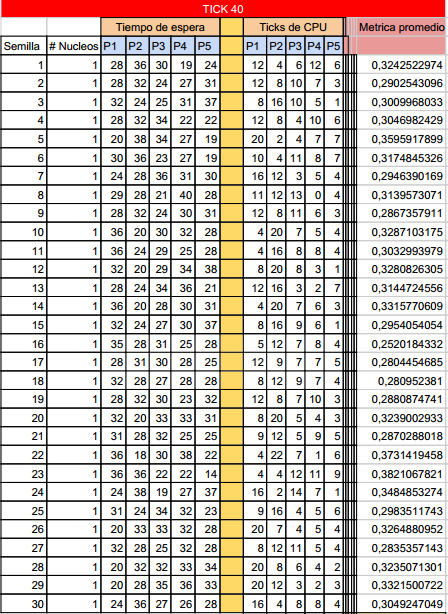
\includegraphics[width=0.7\textwidth]{img/foto1.png}
     \caption{Lottery Scheduling con un solo núcleo hasta el tick 40}
\end{center}
\end{figure}


Como puede apreciarse en la tabla, la métrica da valores muy similares para todos los experimentos realizados.
Para ver que relación existe entre estos valores calculamos la varianza, la esperanza y el desvió estándar de la muestra, lo cuales se definen como:
\begin{center}
	Esperanza $=$ $\mu$ $=$ $\bar{X}$ $=$ $\frac{1}{n}$ $*$ $\sum_{i = 1}^{n}(X_i)$\\
	Varianza $=$ $\sigma^{2}$ $=$ $\frac{1}{n}$ $*$ $\sum_{i = 1}^{n} (X_i - \bar{X})^{2}$\\
	Desvió estandar $=$ $\sigma$ $=$ $\sqrt{Varianza}$	
\end{center}

\begin{figure}[H]
\begin{center}
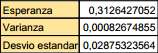
\includegraphics[width=0.4\textwidth]{img/img3.png}
     \caption{Esperanza, varianza y desvió estándar de la métrica promedio}
\end{center}
\end{figure}

Como se puede ver, la varianza y el desvió estándar son muy chicos en comparación con la esperanza.
Numéricamente hablando, la varianza es un $0.26\%$ de la esperanza y el desvió estándar es un $9.20\%$ de la esperanza.

Entonces, como el valor esperado (i.e esperanza) de la métrica se encuentra dentro de un intervalo muy pequeño $(\mu - \sigma, \mu + \sigma)$ $=$ $(0.28,$ $0.34)$, podemos concluir, en base a la experimentación realizada y a la métrica utilizada, que este mismo comportamiento ocurrirá en la mayoría de los experimentos y que, por lo tanto, el \textit{Lottery scheduling} es justo.



\subsubsection{Experimentación con dos núcleos}

En este experimento decidimos llevar a cabo la medición hasta el tick numero 25 del procesador, por los motivos ya dichos anteriormente.
A continuación, los resultados de la experimentación realizada:


\begin{figure}[H]
\begin{center}
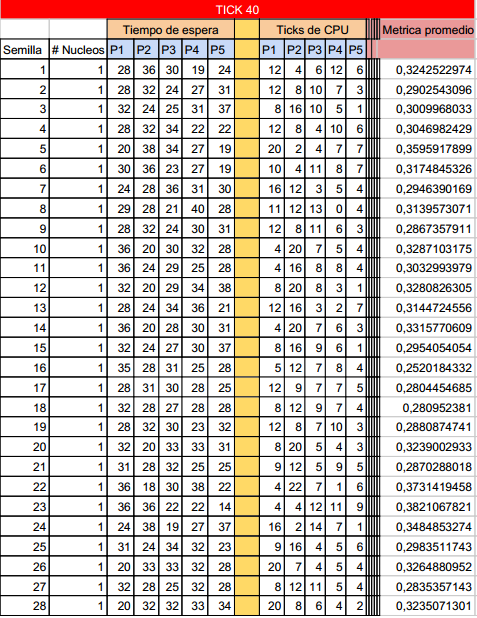
\includegraphics[width=0.6\textwidth]{img/fotaza1.png}
     \caption{Lottery Scheduling con un dos núcleos hasta el tick 25}
\end{center}
\end{figure}

Al igual que sucedió en la experimentación de un solo núcleo, los valores obtenidos con la métrica son muy similares.
Para ver que relación hay entre estos vamos a calcular nuevamente, la esperanza, la varianza y el desvió estándar de la muestra.
Los resultados obtenidos son los siguientes:
\begin{figure}[H]
\begin{center}
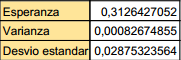
\includegraphics[width=0.4\textwidth]{img/fotaza2.png}
     \caption{Esperanza, varianza y desvió estándar de la métrica promedio}
\end{center}
\end{figure}

Como se puede ver, la varianza es un $2.75\%$ de la esperanza y el desvió estándar es un $15.75\%$ de la esperanza y, el desvió estándar, nos dice que la esperanza se encuentra en el intervalo $(\mu - \sigma, \mu + \sigma)$ $=$ $(0.93$, $1.28)$.
Por esto y por el hecho de que el intervalo en el que se encuentra la esperanza es pequeño, podemos suponer que el resultado obtenido en la experimentación realizada se repetirá en la mayoría de los casos y que, en consecuencia, el \textit{Lottery scheduling} es justo.

\subsubsection{Conclusión}

En general, el Lottery Scheduling se comporta de forma ecuánime, como podemos ver en los experimentos, ya que los intervalos de la esperanza son muy pequeños con ambos núcleos y la varianza también es pequeña. Por otro lado por el factor aleatorio de este algoritmo, es posible que se den casos extremos en donde una tarea o proceso es pospuesto por mucho tiempo o que una tarea gane el uso del CPU muy seguido.